\FloatBarrier
\clearpage
\section{13MeV Proton Irradiated Molybdenum}
\label{appendix:johnmo}

\FloatBarrier
\subsection{Calculation Settings}

\begin{table}[h]
\begin{center}
\begin{tabular}{c c}
\hline\hline
Material & Pure Molybdenum \\
Sheet thickness & 506 micrometers \\
Density & 10,220 $kg m^{3}$ \\
Beam energy & 13MeV \\
Beam projectile & proton \\
Beam current & 5.0 microamps \\
Beam duration & 1500s \\
Simulation end time & 260,000s \\
\hline\hline
\end{tabular}
\end{center}
\caption{}
\label{table:appendixironsettings}
\end{table}

\FloatBarrier
\subsection{Results}

\begin{lstlisting}[style=sOutputFile,caption={Final results for Molybdenum Irradiation},label={listing:activityv2iron}]
23.132      ######################################################
23.132      Sim 1
23.132      ######################################################
23.132      
23.132      Beam flux:          31207545644998.863
23.132      Target depth:       0.000506
23.132      Projectile:         p
23.132      Beam duration/s:    1500.0
23.132      Sim end time/s:     606300.0
23.132      
23.132      Starting Target Material:
23.132      
23.132      ####################################################
23.132                           Isotopes                       
23.132      ####################################################
23.132        Isotope       Percentage by Mass  
23.132        42 Mo 98      24.127937
23.132        42 Mo 96      16.678431
23.132        42 Mo 95      15.917894
23.132        42 Mo 92      14.840324
23.132        42 Mo 100     9.630239
23.132        42 Mo 97      9.555955
23.132        42 Mo 94      9.249221
23.132        
196.630     
196.630     #################################################################
196.630     Particle & Residual Reaction Rates
196.630     #################################################################
196.630     Source isotope: 92Mo  (42092)
196.630     
196.630     
196.630     Source isotope: 94Mo  (42094)
196.630     helium-3:           3.1332823136574574e-12
196.630     deuteron:           26779.397771044376
196.630     triton:             4.691618589935858
196.630     alpha:              35497160.708963595
196.630     gamma:              4046256131.9846444
196.630     proton:             474276321.7635846
196.630     neutron:            2939219987.127653
196.630     94Tc(meta 1):       982541746.5227002
196.630     95Tc(meta 1):       3220288.2361354767
196.630     95Tc:               4316294.073460804
196.630     91Nb:               16990624.30575451
196.630     91Nb(meta 1):       18484514.956021547
196.630     94Tc:               1914038155.7223403
196.630     93Mo:               42473999.299622655
196.630     93Mo(meta 1):       126.22443599491
196.630     94Mo:               431701273.0135327
196.630     90Zr:               18272.130848077595
196.630     
196.630     
196.630     Source isotope: 95Mo  (42095)
196.630     helium-3:           5.46887072783639e-07
196.630     deuteron:           1234961.9156552393
196.630     triton:             41.10937959624232
196.630     alpha:              54324719.08951578
196.630     gamma:              9102804904.23539
196.630     proton:             894337849.3520026
196.630     neutron:            5518562890.307192
196.630     95Tc(meta 1):       1218252833.6464837
196.630     92Nb(meta 1):       33006155.92287399
196.630     96Tc(meta 1):       2679422.9964109
196.630     95Tc:               3689625934.027424
196.630     92Nb:               14122020.720040252
196.631     96Tc:               4182516.45184412
196.631     94Tc(meta 1):       13905093.155669797
196.631     91Nb:               6611098.919676594
196.631     91Nb(meta 1):       576457.3002812921
196.631     94Tc:               59984103.84506015
196.631     95Mo:               439173380.2083463
196.631     94Mo:               456055572.20441234
196.631     
196.631     
196.631     Source isotope: 96Mo  (42096)
196.631     helium-3:           5.5873148279970936e-15
196.631     deuteron:           89980.87611341325
196.631     triton:             146.48193254666154
196.631     alpha:              16359850.77593771
196.631     gamma:              11880347277.430742
196.631     proton:             319281355.5874101
196.631     neutron:            6458872187.0255995
196.631     93Nb:               10952560.277578255
196.631     97Tc:               5027859.164271742
196.631     96Tc(meta 1):       2314902593.6163425
196.631     97Tc(meta 1):       2657069.708104688
196.631     96Tc:               2988618887.151654
196.631     93Nb(meta 1):       5392146.865275863
196.631     89Y:                4.699677647993188
196.631     89Y(meta 1):        0.024318699111099025
196.631     95Tc(meta 1):       186850567.4939038
196.631     92Nb(meta 1):       2991.5174685434013
196.631     95Tc:               387490658.45324874
196.631     92Nb:               2926.3241012165836
196.631     96Mo:               313532526.5135967
196.631     95Mo:               5619671.213466896
196.631     
196.631     
196.631     Source isotope: 97Mo  (42097)
196.631     helium-3:           2.6147848182753646e-08
196.631     deuteron:           1162205.9105530165
196.631     triton:             185.73563697784863
196.631     alpha:              10097428.581276963
196.631     gamma:              6269889067.613607
196.631     proton:             197692275.39840198
196.631     neutron:            4202157441.703513
196.631     97Tc:               2012907421.2696567
196.631     94Nb(meta 1):       7124606.3063902855
196.631     97Tc(meta 1):       515939120.74455863
196.631     90Y:                0.0007502229001053001
196.631     94Nb:               2737836.422765725
196.631     90Y(meta 1):        5.501140264263349e-05
196.631     93Nb:               173177.71086113452
196.631     96Tc(meta 1):       293382016.0592189
196.631     96Tc:               530173961.5847317
196.631     93Nb(meta 1):       40771.640492079096
196.631     98Tc:               2366306.0908124447
196.631     97Mo:               172514065.24175954
196.631     96Mo:               26186498.548734967
196.631     
196.631     
196.631     Source isotope: 98Mo  (42098)
196.631     
196.631     
196.631     Source isotope: 100Mo  (42100)
196.631     
216.077     Gamma Dose - Beam End  
216.077     ===================================================
216.077     Activity (Bq)              1.2188e+09  
216.077     Gamma Energy (eV)          7.0916e+14    
216.077     Gamma Energy (mW)          1.1362e-01   
216.077     Absorbed Dose (mGy/s)      1.1299e-10    
216.077     Absorbed Dose (mGy/hr)     4.0676e-07                
216.077     
216.077     
216.077     Gamma Dose - Sim End
216.077     ===================================================
216.077     Activity (Bq)              6.0485e+06
216.077     Gamma Energy (eV)          1.4080e+13    
216.077     Gamma Energy (mW)          2.2558e-03     
216.077     Absorbed Dose (mGy/s)      2.2433e-12     
216.077     Absorbed Dose (mGy/hr)     8.0757e-09   
216.077     
216.077     
216.077     Absorbed Dose Calculations
216.077     ===================================================
216.077     Absorbed dose assumptions:
216.077     1. radiation from point, emitted isotropically
216.077     2. 80Kg human
216.077     3. 1m from point source
216.077     4. 1m squared surface area
216.077     5. all energy absorbed
216.077     
216.077     
216.077     Dose Limits
216.077     ===================================================
216.077     employees 18+             20 millisieverts/year
216.077     trainees 18+              6 millisieverts/year
216.077     public and under 18s      1 millisievert/year
216.077     public and under 18s      1.140771128E-04 millisieverts/hour
216.077     public and under 18s      3.2E-08 millisieverts/second
216.077     
216.077     Dose averaged over area of skin not exceeding 1cm2
216.077     Source: http://www.hse.gov.uk/radiation/ionising/doses/
216.077     
216.077     1mW gammas completely absorbed by 80kg human will give public limit for entire year over 80 seconds.
216.077     
216.077     Dose under 1W gammas absorbed for 1s no imediate changes (under 100 Rads)
216.077     Dose 1W-2W gammas absorbed for 1s acute radiation syndrome (100-200 Rads)
216.077     Dose 10W+ gammas absorbed for 1s mostly fatal (1000+ Rads)
\end{lstlisting}



\FloatBarrier
\clearpage

\subsection{Total Decay Rates Over Time}

\begin{figure}[htb]
\centering
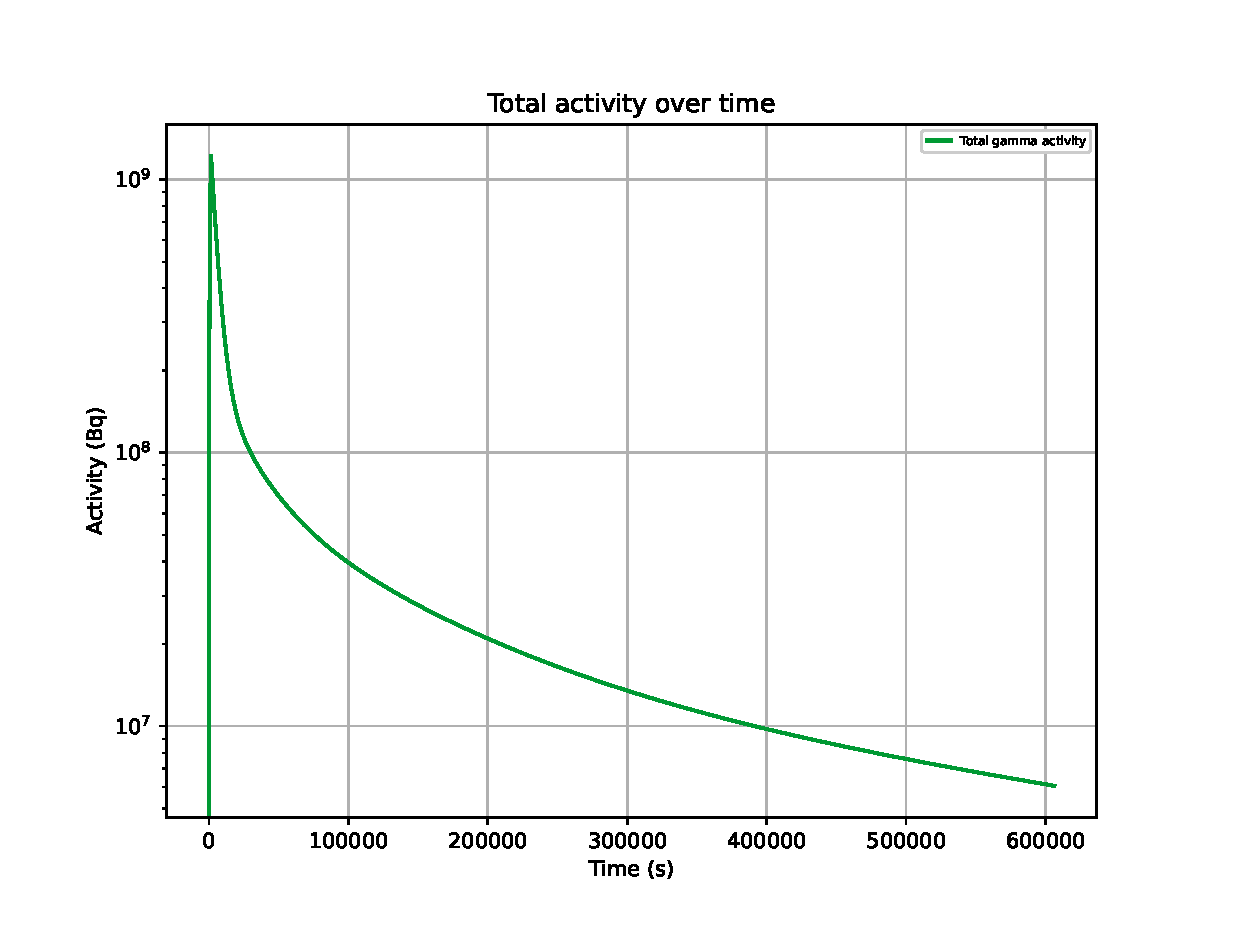
\includegraphics[width=0.5\linewidth]{chapters/results_activity_code/mo-john-hewett/thick/totals/total_activity.eps}
\caption{Total activity over time}
\label{fig:mototalactivity}
\end{figure}

\begin{figure}[htb]
\centering
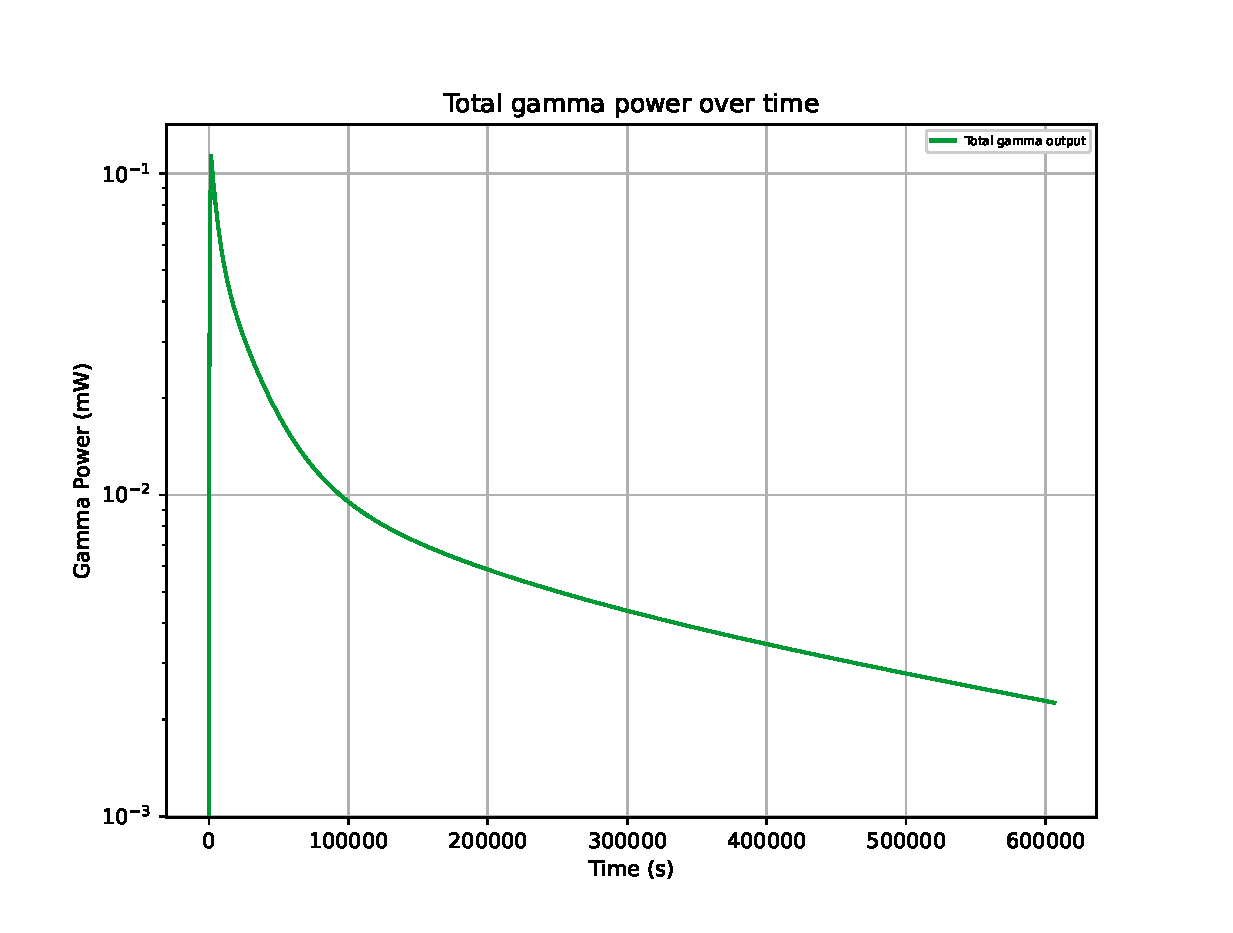
\includegraphics[width=0.5\linewidth]{chapters/results_activity_code/mo-john-hewett/thick/totals/total_gamma_power_mw.eps}
\caption{Total gamma power output over time}
\label{fig:mototalgammaoutput}
\end{figure}



\FloatBarrier
\clearpage

\subsection{Residual Activity Tallied by Target Isotope}

\begin{figure}[htb]
\centering
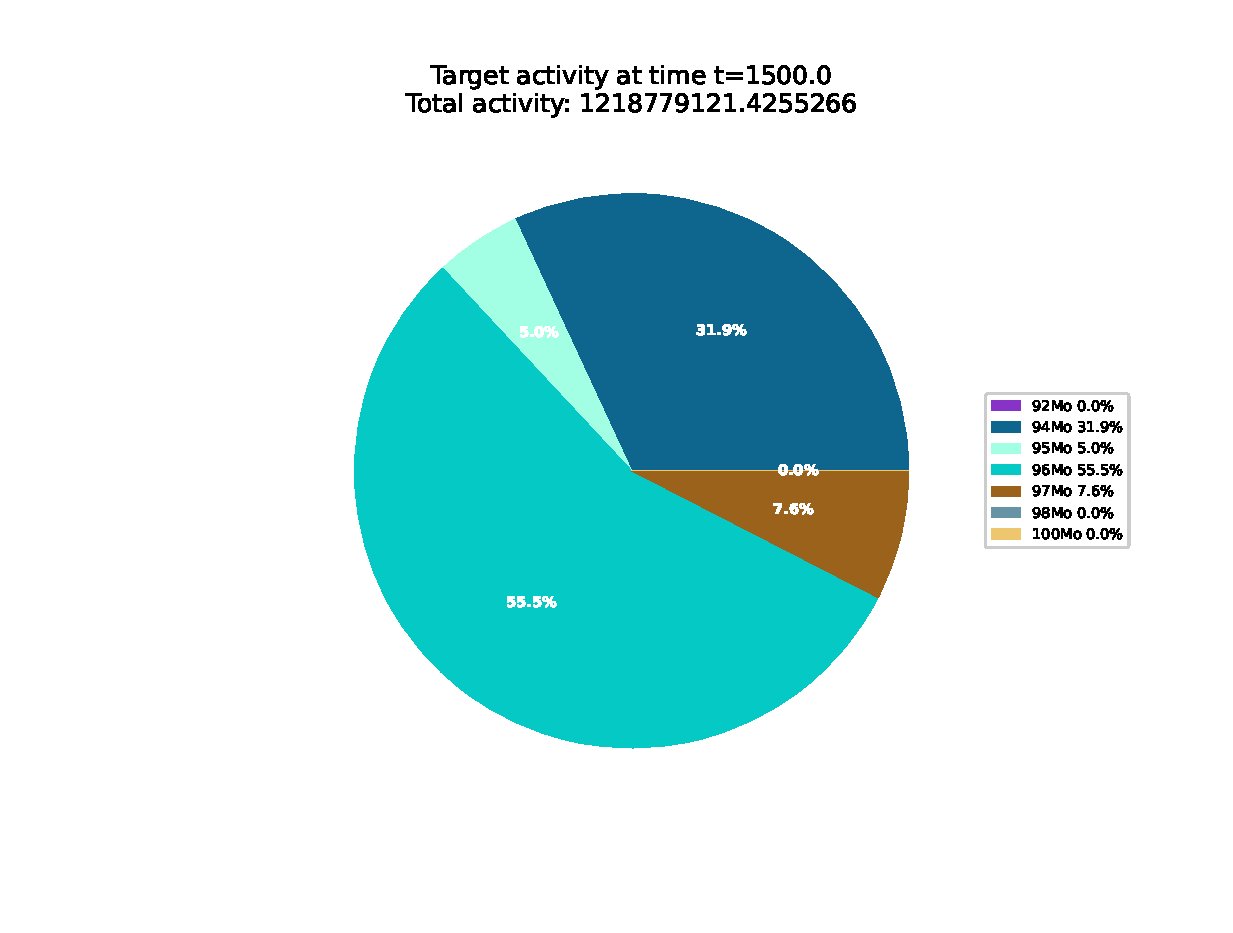
\includegraphics[width=0.5\linewidth]{chapters/results_activity_code/mo-john-hewett/thick/target-activity/0100_1500.eps}
\caption{Radioactive decay from residual isotopes tallied by target isotope - end of beam (1,500 seconds)}
\label{fig:motargetisotopes1500s}
\end{figure}

\begin{figure}[htb]
\centering
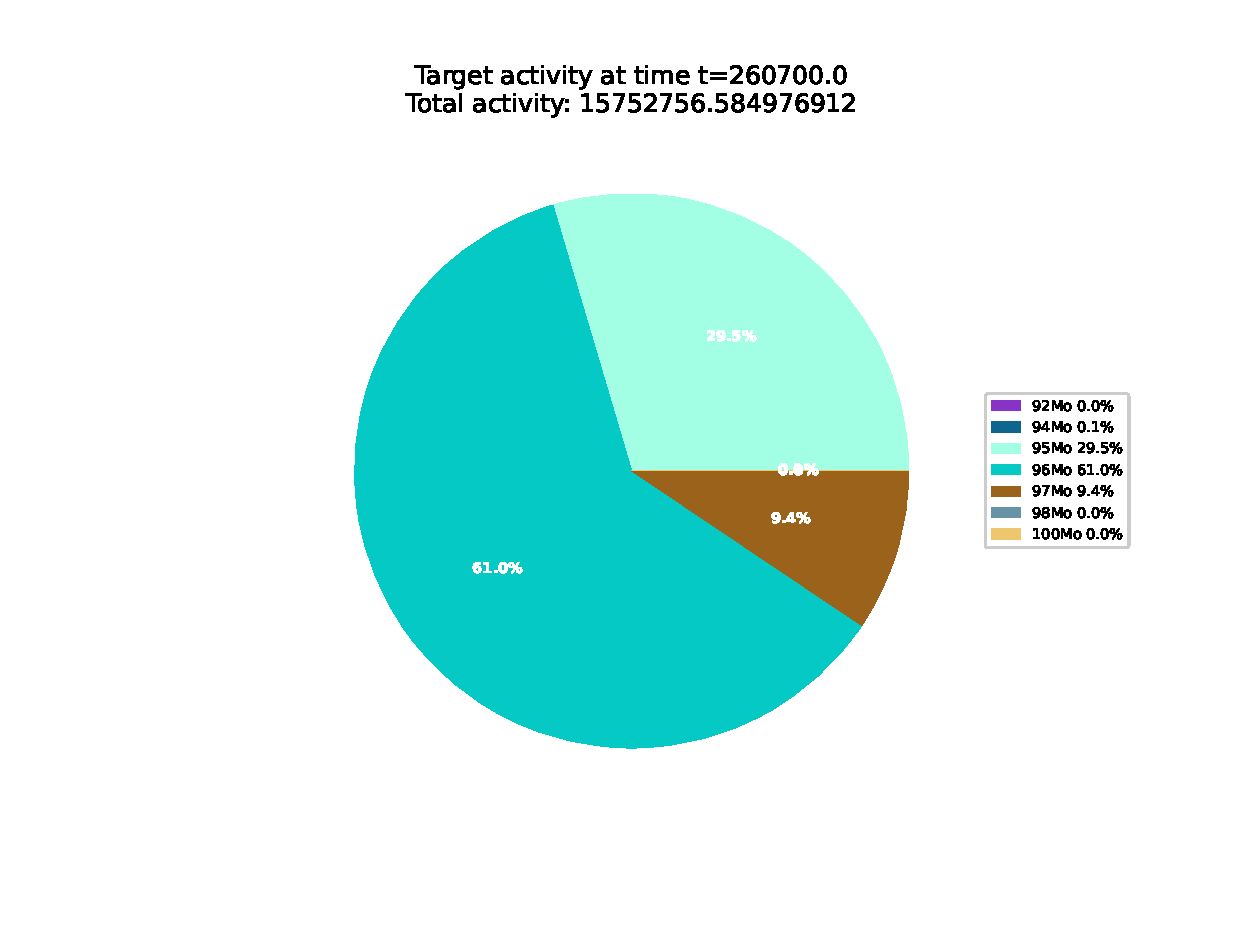
\includegraphics[width=0.5\linewidth]{chapters/results_activity_code/mo-john-hewett/thick/target-activity/0400_260700.eps}
\caption{Radioactive decay from residual isotopes tallied by target isotope - 3 days after irradiation}
\label{fig:motargetisotopes3days}
\end{figure}


\FloatBarrier
\clearpage

\subsection{Residual Activity Tallied by Residual Isotope}

\begin{figure}[htb]
\centering
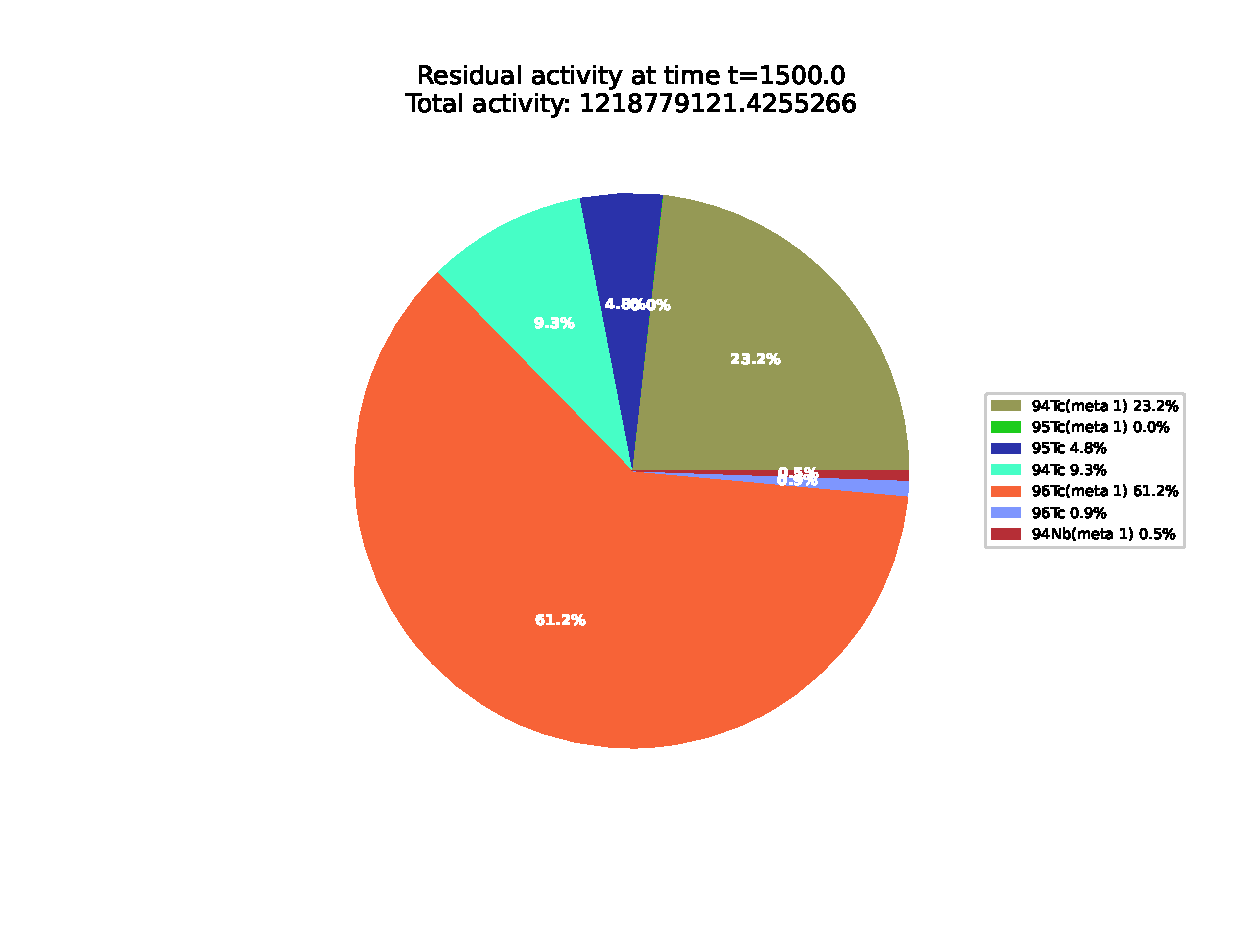
\includegraphics[width=0.5\linewidth]{chapters/results_activity_code/mo-john-hewett/thick/residual-activity/0100_1500.eps}
\caption{Radioactive decay from residual isotopes tallied by residual isotope - end of beam (1,500 seconds)}
\label{fig:moresidualisotopes1500s}
\end{figure}

\begin{figure}[htb]
\centering
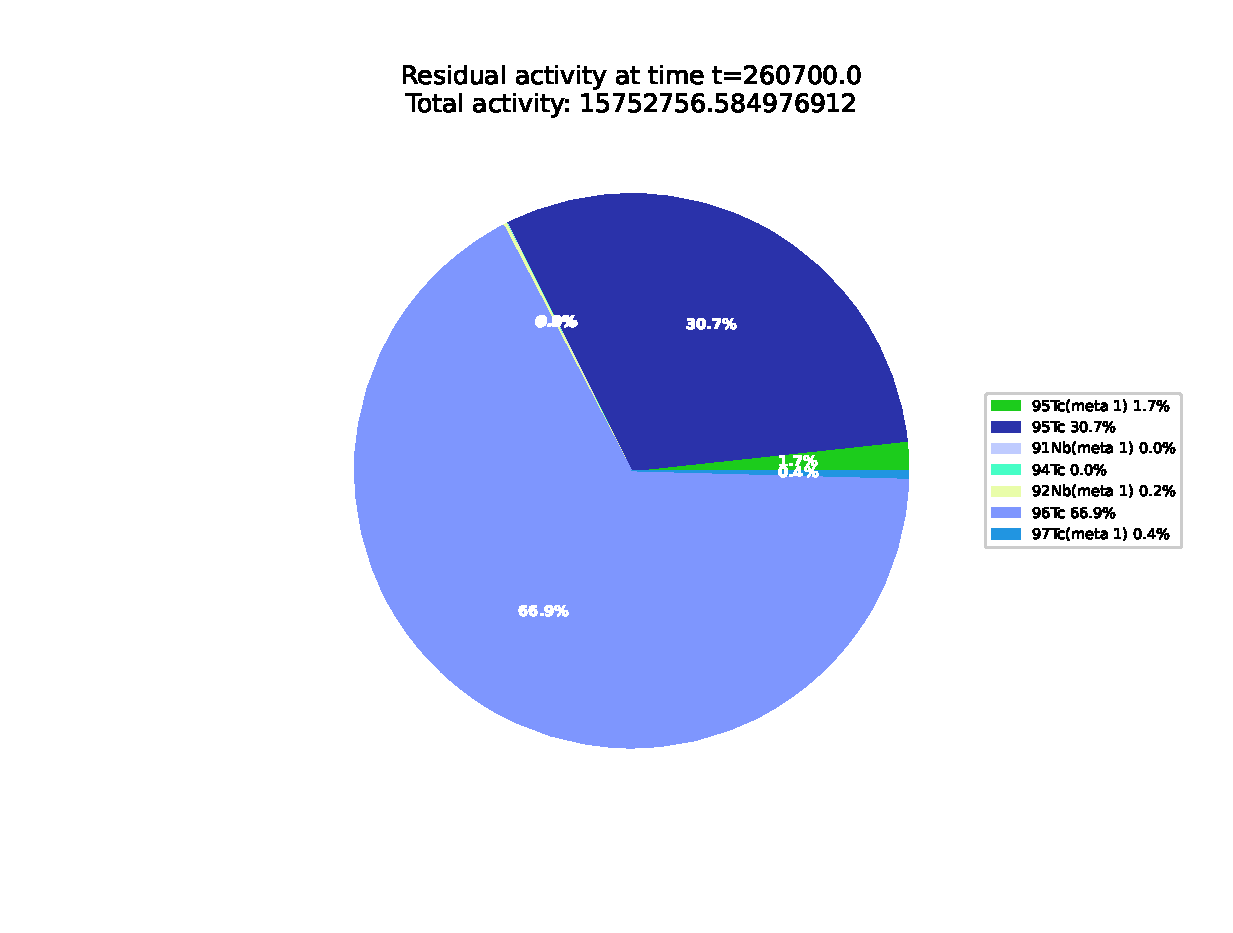
\includegraphics[width=0.5\linewidth]{chapters/results_activity_code/mo-john-hewett/thick/residual-activity/0400_260700.eps}
\caption{Radioactive decay from residual isotopes tallied by residual isotope - 3 days after irradiation}
\label{fig:moresidualisotopes3days}
\end{figure}



\subsection{Residual Gamma Energy Tallied by Residual Isotope}

\begin{figure}[htb]
\centering
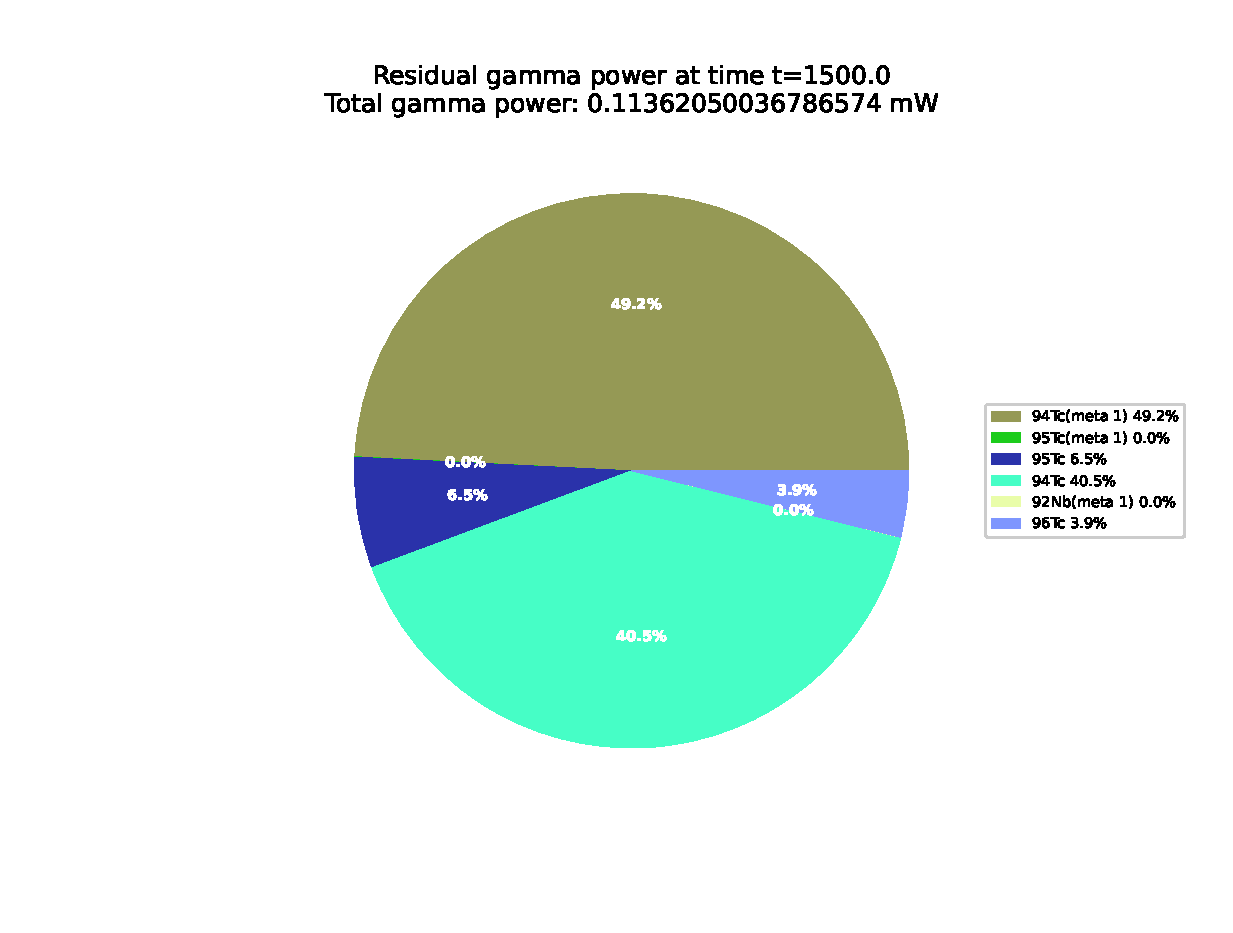
\includegraphics[width=0.5\linewidth]{chapters/results_activity_code/mo-john-hewett/thick/residual-gamma-energy/0100_1500.eps}
\caption{Radioactive decay from residual isotopes tallied by residual isotope - end of beam (1,500 seconds)}
\label{fig:moresidualenergy1500s}
\end{figure}

\begin{figure}[htb]
\centering
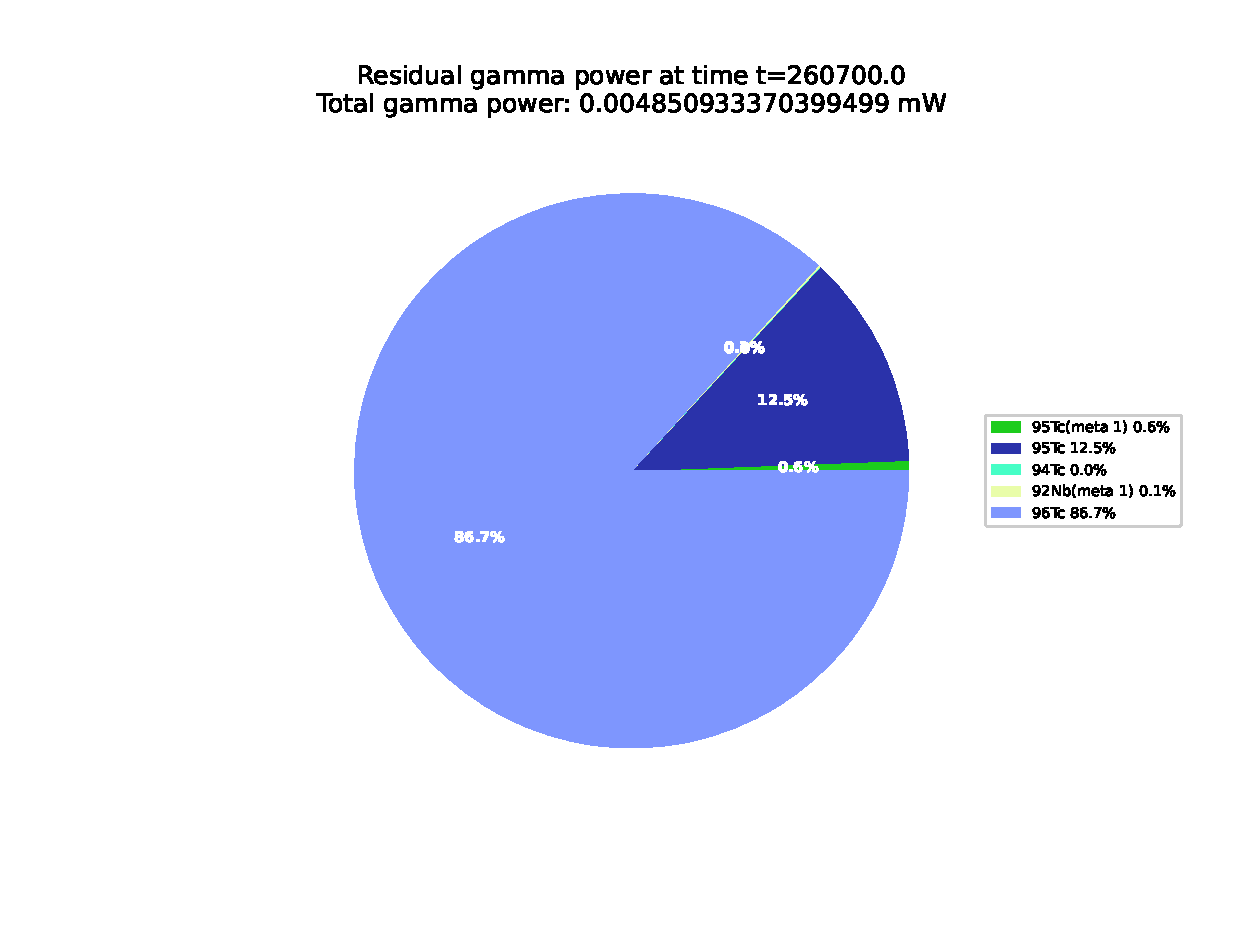
\includegraphics[width=0.5\linewidth]{chapters/results_activity_code/mo-john-hewett/thick/residual-gamma-energy/0400_260700.eps}
\caption{Radioactive decay from residual isotopes tallied by residual isotope - 3 days after irradiation}
\label{fig:moresidualenergy3days}
\end{figure}



\FloatBarrier
\clearpage

\subsection{Gamma Lines}

\begin{figure}[htb]
\centering
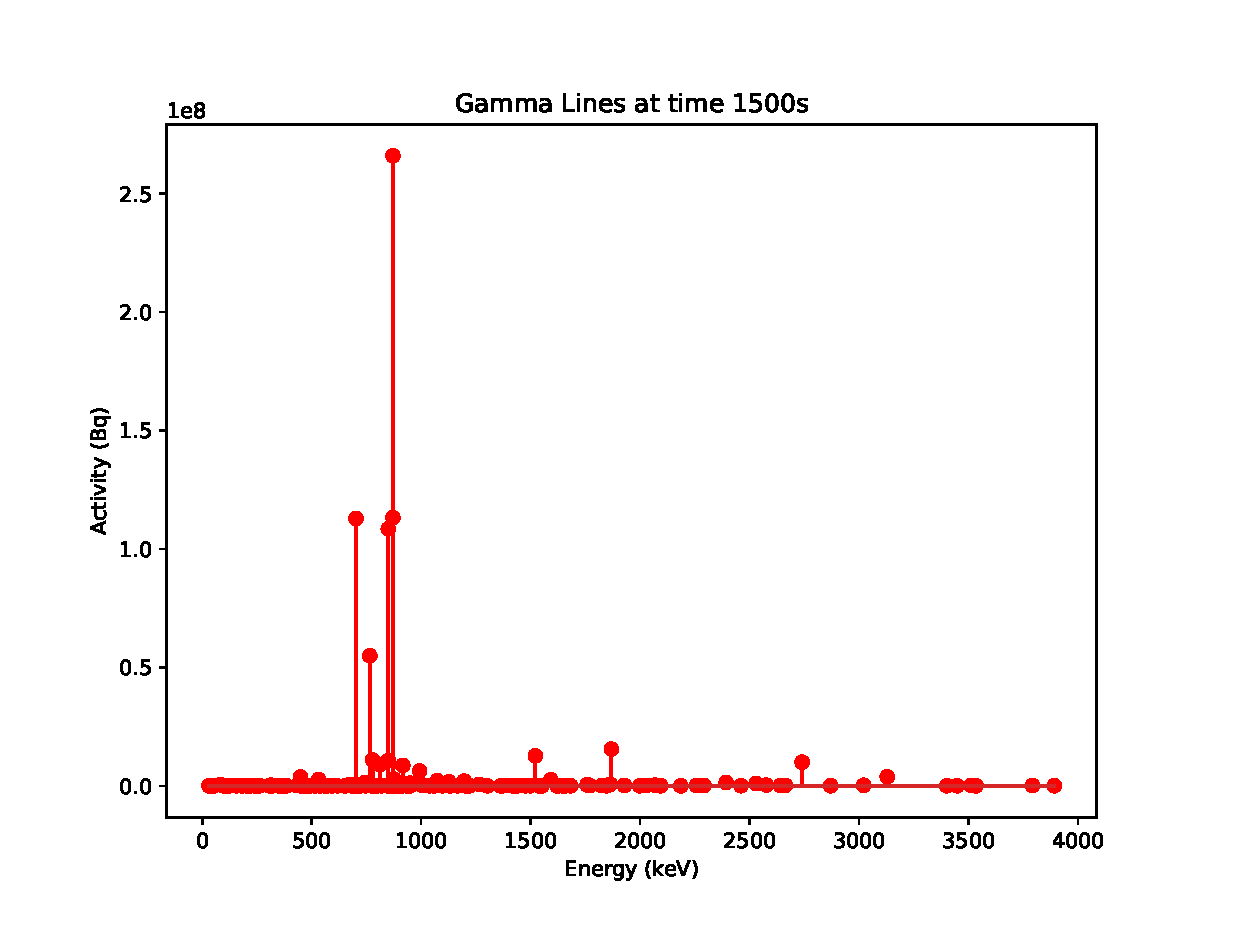
\includegraphics[width=0.5\linewidth]{chapters/results_activity_code/mo-john-hewett/thick/gammas/0100_1500.eps}
\caption{Predicted gamma lines - end of beam (1,500 seconds)}
\label{fig:mogammalines1500s}
\end{figure}

\begin{figure}[htb]
\centering
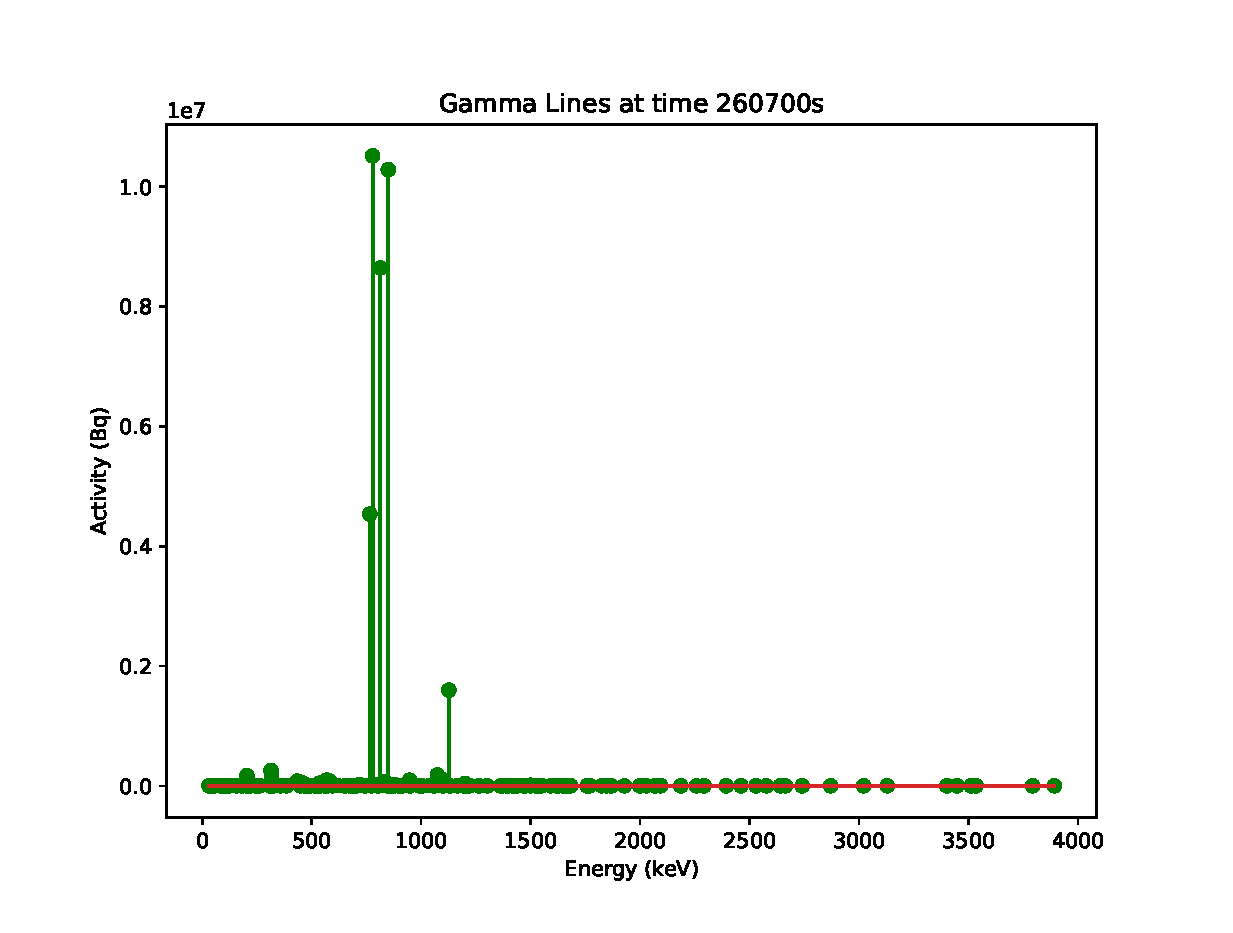
\includegraphics[width=0.5\linewidth]{chapters/results_activity_code/mo-john-hewett/thick/gammas/0400_260700.eps}
\caption{Predicted gamma lines - 3 days after irradiation}
\label{fig:mogammalines3days}
\end{figure}



